\chapter{Background}

%-------------------------------------------------------------------------------
% SECTION: Radiance
%-------------------------------------------------------------------------------
\section{Radiance}
\label{sec:radiance}

Radiance is a general term for the amount of light energy being transmitted through an area on a surface in a specific direction. Or more simply as the measure of brightness and color of a single ray of light \cite{bib:rtr}.

In order to understand how to calculate radiance, we must first understand radiant flux and flux density. Radiant flux, $\phi$, is a measure of energy (measured in joules) per second. Flux density is the instantaneous amount of radiant flux over an area, and is written as:
\begin{equation}
E = \frac{d\phi}{dA}
\label{eqn:flux_density}
\end{equation}
We can now define radiance as the flux density with respect to a projected area and a solid angle, or:
\begin{equation}
L = \frac{d^{2}\phi}{dA*\cos\theta*dw}
\label{eqn:radiance}
\end{equation}
Incoming radiance, or irradiance, is the radiance arriving at a surface, or the flux density of arriving light. We can define this in terms of radiance, where $x$ is a surface point and $w$ is the incoming ray direction, as:
\begin{equation}
E(x,w) = L(x,w) * \cos\theta * dw
\label{eqn:irradiance}
\end{equation}
Further more, we integrate over a hemisphere to solve for the incoming radiance, at point $x$, in all directions:
\begin{equation}
E(x) = \int L(x,w) * \cos\theta * dw
\label{eqn:irradiance_integral}
\end{equation}
Ultimately we are interested in the reflected radiance: the amount of irradiance that is reflected by a surface back towards our virtual camera. This is based on the material properties of the surface, which is typically represented by a BRDF (bi-direction reflectance distribution function). BRDFs are defined per-surface, and represented as $f(x, w^{\prime}, w)$. They solve for the ratio of radiance that is transmitted from an incoming direction, $w^{\prime}$, to an outgoing direction, $w$, at a surface point, $x$ (see figure \ref{fig:incoming_radiance}). Incorporating the BRDF, the equation for reflected radiance is:
\begin{equation}
L(p) = \int f(x, w^{\prime}, w) * L(p,w) * \cos\theta * dw
\label{eqn:radiance_integral}
\end{equation}

\begin{figure}
   \centering
   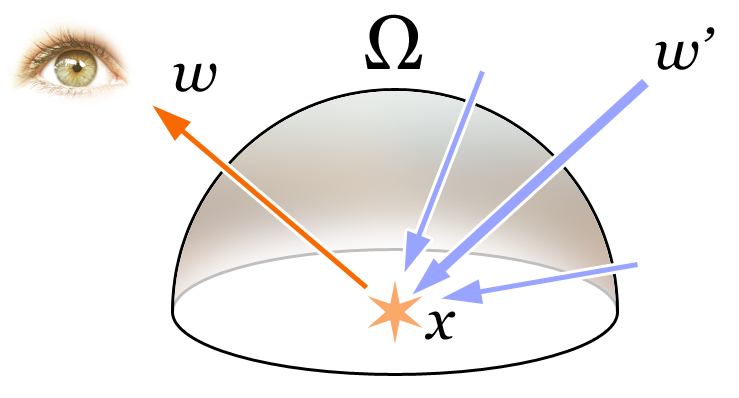
\includegraphics[width=100mm]{../img/rendering-equation-image.png}
   \captionfonts
   \caption[Incoming radiance hemisphere]{Incoming radiance in a hemisphere about a point, reflecting towards the camera. \cite{bib:nikishin_radiance}}
   \label{fig:incoming_radiance}
\end{figure}

%-------------------------------------------------------------------------------
% SECTION: Phong Reflection Model
%-------------------------------------------------------------------------------
\section{Phong Reflection Model}
\label{sec:phong_model}

The Phong reflection model is a simplified shading model used to calculate reflected radiance from one light source. It is most commonly used in scenarios that require fast computation, such as real-time graphics applications. It was presented by Phong in his University of Utah Ph.D. dissertation in 1973 \cite{bib:phong_thesis}. The equation calculates the reflected radiance using three color-vector terms: an ambient, diffuse, and specular.

The ambient component represents indirect illumination as a constant amount of reflected radiance added to all shaded points. This is the simplest term, but also poorly represents the subtleties of indirect illumination.

The diffuse component represents direct illumination using Lambertian reflectance of the incoming radiance. Lambertian refers to Lambert's cosine law, which states that, for perfectly diffuse surfaces, the diffuse reflected radiance is proportional to the cosine of the angle between the surface normal and the view vector, $\theta_{i}$. Figure \ref{fig:phong} visualizes these components.

\begin{figure}
   \centering
   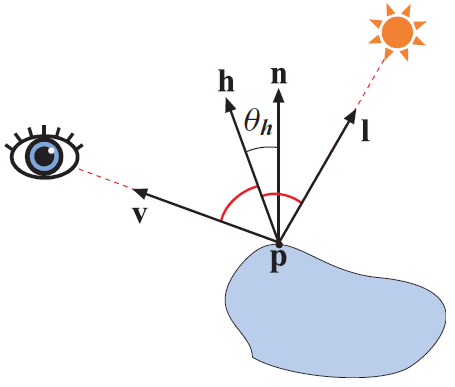
\includegraphics[width=100mm]{../img/RTR3_05_13_phong.png}
   \captionfonts
   \caption[Phong Shading Vectors]{The vectors involved in the Phong Reflectance Model. \cite{bib:rtr}}
   \label{fig:phong}
\end{figure}

The specular component represents the shininess we can view from certain angles on highly reflective surfaces. Specular reflectance is calculated by raising the cosine of the angle between the surface normal and the half vector (the vector halfway between the view and light vector), $\theta_{h}$, to the shininess of the surface, $s$.

Each of these components represent the ratio of incoming radiance, $C_{light}$ to reflected radiance, $C_{out}$, but the reflected radiance is also scaled by the surface material’s color characteristics, $C_{mat}$, as well as ambient, diffuse, and specular characteristics (represented by the scalar ratios: $M_{amb}$, $M_{diff}$, and $M_{spec}$, respectively). Combining these components we get the final Phong reflection model equation:
\begin{equation}
C_{out} = (M_{amb} * C_{mat} * C_{light}) + ((n \cdot l) * M_{diff} * C_{mat} * C_{light}) + ((n \cdot h) ^s * M_{spec} * C_{mat} * C_{light})
\label{eqn:phong}
\end{equation}

%-------------------------------------------------------------------------------
% SECTION: Anti-aliasing
%-------------------------------------------------------------------------------
\section{Anti-aliasing}
Anti-aliasing combats aliasing, the artifacting caused by under-sampling. A typical example of this in signal processing, where an analogue signal is sampled as some rate to determine it’s amplitude at that point in time. If the sample rate is too low (i.e. under-sampling) then the signal will not be accurately captured because the signal’s characteristics between samples was lost. This can be seen in Figure \ref{fig:undersampling}.

\begin{figure}[h!]
   \centering
   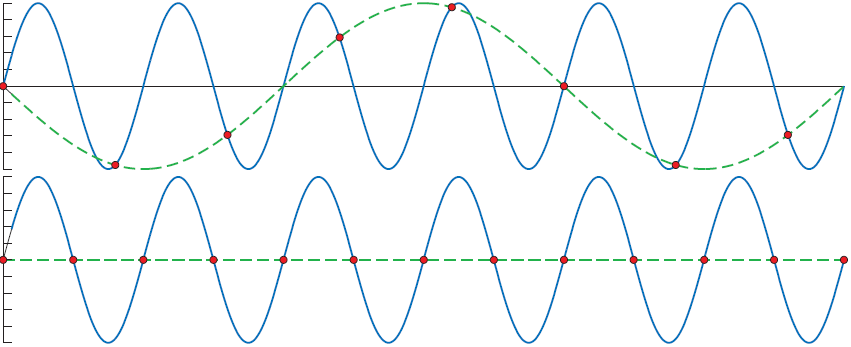
\includegraphics[width=100mm]{../img/RTR3_05_21_undersampling.png}
   \captionfonts
   \caption[Signal Undersampling]{The blue signals are being undersampled by the red dots, which leads to inaccurate reconstruction as evidenced by the dotted green line. \cite{bib:rtr}}
   \label{fig:undersampling}
\end{figure}

This occurs in computer graphics due to the limited sample rate provided by our display devices. To illustrate this point, imagine attempting to display a sphere with four pixels. More typically we experience aliasing in computer graphics as “jaggies,” or lines that should be smooth but are jagged (see Figure \ref{fig:jaggies}).

\begin{figure}[h!]
   \centering
   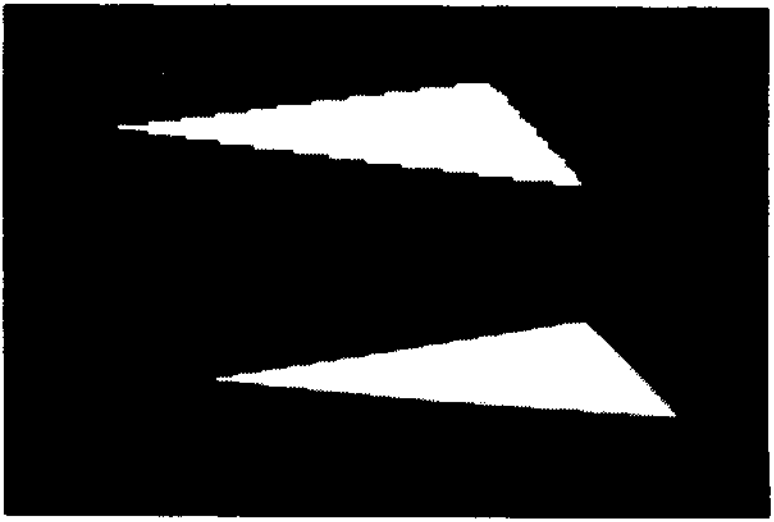
\includegraphics[width=100mm]{../img/jaggies.png}
   \captionfonts
   \caption[Jaggies]{Jagged edges apparent along the silhouette edges of the top triangle are reduced via anti-aliasing techniques in the lower triangle \cite{bib:crow1977}.}
   \label{fig:jaggies}
\end{figure}

In order to combat this phenomenon, techniques for anti-aliasing have been developed. These can take many forms \cite{bib:jimenez2011}, but generally it involves some form of over-sampling (i.e. rendering the image at a multiple of the display resolution) to compensate for the fixed sample rate of our display devices. By over-sampling the rendering, we can capture the subtleties of the image in software, and can down-sample the image in a way that helps alleviate the fixed display sample rate.

The simplest form of this technique is called super-sampling: where we render an image at some multiple of the desired final resolution, and down-sample the large image back to the desired final resolution by averaging the extra pixels into one value. For example, if we wish to render a 300 by 300 pixel image, we might render an intermediate image at 600 by 600 and then each final pixel is represented by 4 intermediate pixels, which can be averaged into one final pixel value; this is called 4x super-sample anti-aliasing.

However, in order to reduce the aliasing artifacts to an acceptable level, we usually require a large super-sample rate. This can result in unacceptably long render times. The main reason we require high super-sample rates in ray-tracing is the regular pattern  created by generating rays that pass through the center of each pixel. Generally in ray-tracing, the more random you can make a sample pattern (while not missing important features), the less aliased your final image will be. Therefore, we randomly jitter the direction of each ray within the bounds of the pixel. This facilitates lower super-sample rates.

An example image of anti-aliasing in our rendering algorithm can be seen in Figure \ref{fig:anti-aliasing}.

\begin{figure}[h!]
    \centering
    \subfloat[No Anti-aliasing]{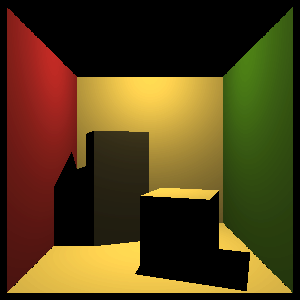
\includegraphics[width=70mm]{../img/cornell_simp_noAA.png}}
    ~
    \subfloat[9x Anti-aliasing]{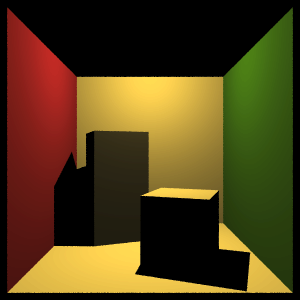
\includegraphics[width=70mm]{../img/cornell_simp_9xAA.png}}
    \caption[Anti-aliasing comparison]{Our simple Cornell box rendered with no anti-aliasing, and 9x box-filtered anti-aliasing.}
    \label{fig:anti-aliasing}
\end{figure}

%-------------------------------------------------------------------------------
% SECTION: Monte Carlo Integration
%-------------------------------------------------------------------------------
\section{Monte Carlo Integration}
\label{sec:monte_carlo_integration}

Monte Carlo integration is a technique used to evaluate integrals \cite{bib:pbr}. By repeatedly evaluating randomized discrete samples, we converge on the true evaluation of the integral. On average, these evaluations correspond to the correct solution, therefore we average multiple runs of the algorithm. We do not arrive at the correct solution in this way, but one that is statistically close.

We use Monte Carlo to evaluate the complex integral in Equation \ref{eqn:radiance_integral}. It is almost impossible to create a closed-form representation of the terms in this equation, and therefore Monte Carlo lends itself to its evaluation. To evaluate the incoming radiance at a point, we can generate randomized sample vectors (rays) over the domain of integration, the unit hemisphere. We then average these samples in order to obtain a result that is close to the true evaluation.

The main drawback of Monte Carlo integration is that it only converges at a rate of $O(n^{-1/2})$, with n being the number of discrete random samples. This means that increasing the number of samples by 4 would only reduce the error by half \cite{bib:pbr}. And because each sample requires one or more rays to be traced against the scene geometry and shaded at their intersection point, it quickly becomes cost-prohibitive to obtain low-error results. Error in this technique is exhibited by adjacent pixels that have disparity in their brightness and color, or noise.

Most of the current research in Monte Carlo for computer graphics is aimed at reducing this error through methods other than increasing the sample count \cite{bib:pbr}. One technique we use to better distribute the sample rays across the unit hemisphere is to discretize the hemisphere into a grid of sample directions with higher density in areas of higher importance, namely the top of the hemisphere where the $n \cdot l$ factor is largest, and jitter each sample direction by a random amount.

%-------------------------------------------------------------------------------
% SECTION: CPU versus GPU
%-------------------------------------------------------------------------------
\section{CPU versus GPU}
\label{sec:cpu_v_gpu}

due to their purpose. The CPU is considered a serial processor that handles general computation, which is typically thought of as instruction-driven, and involves executing unpredictable instructions on irregular data and likely includes branching. The GPU, on the other hand, is a stream processor optimized for data-driven graphics rendering of more regular data with predictable memory access. \cite{bib:rtr}

Because of their differing purposes, the CPU and GPU have traditionally been divided into two physically separate components of a computer system’s architecture connected by the PCI bus. The application running on the CPU will transmit rendering data and instructions over this bus to the GPU, which will process this input and produce a rendering. Depending on the purpose of this rendering, it can either be displayed on a monitor attached directly to the GPU, or transmitted back over the bus to the CPU for additional processing. As is common in multiprocessing systems, the two common problems we experience are load balancing and communication \cite{bib:rtr}. 

Load balancing can take place between the CPU and GPU, as well as internally within the GPU. The programmer is generally responsible for handing the load balancing between these two components, while the GPU itself leverages FIFO queues between stages to avoid stalling any part of the pipeline.

The latency and bandwidth of the bus connecting the CPU and GPU can cause communication problems as well. The theoretical maximum one-way bandwidth of the PCI Express 2.0 bus is 8.0 GB/s \cite{bib:pci_press}, while if we wanted to render 300 million triangles per second we would require a rate of 10.2 GB/s just to transfer the triangles to the GPU \cite{bib:rtr}. If we want to saturate this bandwidth, we must be constantly streaming data across the bus, however this is not always the use-scenario. Many times we wish to transmit data to the GPU, process it, and send it back to the CPU. In this case, the PCI bus can become the bottleneck as it is designed for one-way streaming of data.

%-------------------------------------------------------------------------------
% SECTION: Heterogenous Chip Architectures
%-------------------------------------------------------------------------------
\section{Heterogenous Chip Architectures}
\label{sec:heterogenous_chips}

The traditional architecture for systems with both CPU and GPUs involves the PCI bus, which connects two these two disparate components. However, recent advancements have allowed chip densities so high that both CPU and GPU can fit onto one silicon chip. These architectures, that combine CPU and GPU, are called heterogenous chips.

Intel has released both Sandy Bridge and, more recently, Ivy Bridge architectures \cite{bib:intel_press} that adhere to this ethos, and AMD has released Fusion \cite{bib:amd_press}. By combining both the CPU and GPU onto one chip, the hardware can bypass the shortcomings of the PCI bus to more quickly communicate.

In systems utilizing the traditional architecture, rendering small scenes that require final data processing on the CPU would have been cost-prohibitive due to the latency required to transfer data from CPU to GPU and back again. However, with heterogenous chip architectures, we can almost ignore this latency in our algorithms; allowing for new-found simplicity.

